\documentclass[11pt]{article}

\usepackage[margin=0.95in]{geometry}
\usepackage{microtype}
\usepackage{booktabs}
\usepackage{array}
\usepackage{xcolor}
\usepackage{enumitem}
\usepackage[hidelinks]{hyperref}
\usepackage{caption}
\usepackage{pgfplots}
\pgfplotsset{compat=1.17}
\captionsetup{font=small, labelfont=bf}

\definecolor{ink}{HTML}{1D2129}
\definecolor{accent}{HTML}{1A5FB4}
\definecolor{good}{HTML}{2E7D32}
\definecolor{bad}{HTML}{B3261E}
\definecolor{warn}{HTML}{8A4600}

\newcommand{\code}[1]{\texttt{#1}}

\title{\vspace{-1.2em}The Skateboard: Early Trials\\
\large AI-assisted Fortran$\to$GPU porting across four models\vspace{-0.4em}}
\author{Companion to \texttt{skateboard.tex} and \texttt{architecture.tex}}
\date{July 30, 2026}

\setlength{\parskip}{0.35em}

\begin{document}
\maketitle
\vspace{-1.2em}

\section{What these trials are}

We ran the skateboard harness (see \code{architecture.tex}) on one porting task
and four AI models. The task: take one Fortran subroutine that advances the
non-linear one-dimensional shallow water equations by a time step, and make it
run on an NVIDIA GPU without changing what it computes. Each model's output is
driven through a fixed gate sequence---build, GPU device-execution proof,
memory/race sanitizer, correctness on visible data, timing, then correctness on
a held-out dataset the model never sees. The agent may edit exactly one file;
everything that judges its work is out of its reach.

Two studies are reported. The \emph{model matrix} runs four models once each
(up to three repair attempts). The \emph{iteration study} gives the weakest
model, a locally-served 14-billion-parameter model, twenty attempts, to see
whether persistence substitutes for capability.

\section{The constraints the port must satisfy}

Every claim below is enforced mechanically by a component the model cannot edit.

\paragraph{The code and the dialect.}
The target is chapter~4 of the \emph{Modern Fortran} ``tsunami'' example
(Curcic). It is Fortran~2008: \code{iso\_fortran\_env} 32-bit reals
(\code{real32}), assumed-shape array arguments, and \emph{standard parallelism}
via \code{do concurrent}. The original kernel is written in whole-array form and
calls an array-valued function for the 2nd-order centered difference. The port
target is a single subroutine, \code{step(h,u)}, that updates water height
\code{h} and velocity \code{u} in place; the momentum update is computed first
from the old fields, then the continuity update uses the freshly-updated
velocity and the old height. The agent may modify only \code{src/mod\_kernel.f90}.

\paragraph{What the compiler will accept.}
The build gate is NVIDIA \code{nvfortran} 25.9 invoked as
\code{-O2 -stdpar=gpu -gpu=cc89,mem:managed -Minfo=accel}. Under this flag a
\code{do concurrent} loop is turned into a GPU kernel. The compiler is strict
about what it will offload: it rejected a \code{block} construct placed inside a
\code{do concurrent} (Sonnet's first attempt), and it rejected indexing a
function result as \code{diff\_centered(u)(i)} together with an undeclared loop
variable (qwen's first attempts). Whole-array assignments that call array-valued
functions compile, but run on the host rather than the device. Automatic and
allocatable temporaries are accepted. The compiler flags, the exact command, and
the environment are baked into the builder image; the agent's patch can change
Fortran source only, never how it is compiled.

\paragraph{How the GPU is used.}
The method is ISO standard parallelism, not CUDA and not directives: each
\code{do concurrent} loop nest becomes one CUDA kernel, generated by
\code{nvfortran -stdpar=gpu} for compute capability 8.9 (an RTX~4000 Ada). The
harness does not trust a successful build to mean the code ran on the device. It
sets \code{NVCOMPILER\_ACC\_NOTIFY=1} and counts the ``launch CUDA kernel'' lines
the runtime prints; the device-execution gate fails if that count is zero. A
directive port that silently falls back to the host is therefore caught, not
accepted. NVIDIA \code{compute-sanitizer} (memcheck, racecheck) must also run
clean on the device.

\paragraph{The memory region shared with the GPU.}
Data is shared through CUDA \emph{managed} (unified) memory, requested by
\code{-gpu=mem:managed}. The height and velocity arrays---at the production size,
two million \code{real32} elements, about $8$\,MB each---plus the per-step
difference and flux temporaries are allocated as managed memory. Managed pages
migrate between host and device on demand, at page granularity, and stay
resident on the device across successive kernel launches as long as only the GPU
touches them. This detail decides performance: a port that keeps the arrays on
the device between steps runs fast, whereas a port that also performs a
whole-array copy on the host (for example \code{h\_old = h} or \code{u = u\_new})
forces those two-million-element arrays to migrate host$\leftrightarrow$device
every step, and pays for it (Section~\ref{sec:results}).

\paragraph{What the oracle accepts.}
Correctness is decided by capture-replay against reference outputs the agent
never sees. For each of five ``visible'' single-step cases the ported kernel is
run and its outputs compared, per variable, to the reference. An element passes
if any of three metrics is within tolerance---absolute
$\le 10^{-6}$, relative $\le 10^{-5}$, or units-in-the-last-place
$\le 16$; a variable passes only if every one of its elements passes. The bands
were calibrated from the spread the CPU code already exhibits between
\code{-O2} and \code{-ffast-math} builds. A separate held-out set of five cases,
generated from a different initial condition, is compared only after every other
gate passes, and the oracle returns pass/fail for it alone---never a numeric
error---so nothing quantitative about the held-out data can leak back to the
agent. The reference outputs, the tolerances, and the comparator live in a
read-only service on a network the agent cannot reach.

\paragraph{The baseline.}
Speed is measured end to end on a production-sized run: the domain is 20{,}000
copies of the 100-point chapter-4 domain laid end to end (two million points),
marched 5{,}000 explicit forward-Euler steps. Because each tile evolves
identically under the periodic scheme, the small single-step cases remain an
exact correctness reference for the large timing run. Two baselines are measured
\emph{before} any model runs: the best CPU configuration of the original
code (\code{nvfortran -O2 -stdpar=multicore}, all cores) and the naive
compiler-only GPU attempt (the unmodified whole-array code compiled with
\code{-stdpar=gpu}). In the model-matrix run these were $10.90$\,s and
$7.95$\,s respectively. Timings are whole-process wall clock and therefore
include CUDA start-up, which is the honest end-to-end number.

\paragraph{The prompt the agent is given.}
The instruction has two fixed parts and one variable part. A single system
prompt states the job and the hard rules, and never changes:

{\small
\begin{verbatim}
You are an expert Fortran/GPU engineer working inside an automated porting
harness.

Your task: port a numerical kernel so it runs on an NVIDIA GPU, WITHOUT
changing what it computes (within a calibrated floating-point tolerance).

Hard rules:
- You may modify ONLY the file src/mod_kernel.f90. Do not touch any other file.
- Preserve the module name (mod_kernel), the public subroutine name and
  signature (`subroutine step(h, u)` with
  `real(real32), intent(inout) :: h(:), u(:)`), and the SEMANTIC CONTRACT
  documented in the file.
- Return the COMPLETE new contents of src/mod_kernel.f90, and nothing else,
  wrapped exactly between a line containing `===BEGIN FILE src/mod_kernel.f90===`
  and a line containing `===END FILE===`. Do not put a Markdown code fence
  inside the markers. Output the raw Fortran only.
- After the END marker you may add a short NOTES: line explaining what you
  changed.
\end{verbatim}
}

\noindent A strategy card names the porting method for the current rung; this is
the card for the \code{do concurrent} rung (the OpenMP-\code{target} rung swaps
in a different card):

{\small
\begin{verbatim}
STRATEGY: standard-parallelism offload.
Rewrite `step` so nvfortran compiled with `-stdpar=gpu -gpu=cc89,mem:managed`
offloads it to the GPU. Replace the whole-array assignments with explicit
`do concurrent (i = 1:n)` loops. Inline the 2nd-order centered difference
(periodic boundaries) from mod_diff::diff_centered directly into the loops.
Because the stencil reads neighbours, use temporary arrays for the differences
so the update is not corrupted in place.
ORDERING (must preserve): compute the new u first from the OLD u and OLD h;
then compute the new h using the FRESHLY-UPDATED u and the OLD h.
\end{verbatim}
}

\noindent The variable part is the current contents of \code{mod\_kernel.f90}
(the file to port), the two read-only context files \code{mod\_diff.f90} and
\code{mod\_params.f90} so the model can see \code{diff\_centered} and the physical
constants, and---on a retry---the model's own previous failing version together
with the structured diagnostic from the gate that rejected it (the compiler
errors, or the comparator's per-variable pass/fail and error magnitudes). Notably
absent: any test input, any reference output, and anything about the held-out
set. The model is told what to produce and why its last try failed, never the
answers it is being checked against.

\section{Results}
\label{sec:results}

\subsection{The model matrix}

Four models, one attempt-ladder each (up to three repair attempts on the
\code{do concurrent} strategy). Table~\ref{tab:matrix} gives the outcome. Two
Claude models produced accepted ports; the Gemini and local models never
produced a numerically correct one. Crucially, no wrong port was ever
accepted---the models that failed did so \emph{at a gate}, with the oracle or
the compiler refusing them, not by the harness overlooking an error.

\begin{table}[htbp]
\centering\small
\begin{tabular}{@{}llccr@{}}
\toprule
\textbf{Model} & \textbf{Backend} & \textbf{Outcome} & \textbf{Attempts} & \textbf{Speedup} \\
\midrule
Claude Opus 4.8   & Anthropic API        & accepted            & 1 & $\mathbf{12.2\times}$ \\
Claude Sonnet 5   & Anthropic API        & accepted            & 2 & $\mathbf{8.9\times}$ \\
Claude Haiku 4.5  & Anthropic API        & accepted (slow)     & 1 & $0.13\times$ \\
Gemini 2.5 Flash  & OpenAI-compat.\ API  & not accepted        & 3 (build) & --- \\
qwen2.5:14b       & local (Ollama)       & not accepted        & 3 (build) & --- \\
\bottomrule
\end{tabular}
\caption{Model matrix. ``Attempts'' is the number used before acceptance, or the
cap with the stage that failed. Opus is from a separate single-model run under
the same setup; the others are one campaign. Speedup is versus the best CPU
configuration.}
\label{tab:matrix}
\end{table}

Three findings sit inside that table.

\textbf{The feedback loop, not raw generation, produced Sonnet's success.}
Sonnet's first attempt failed to build: it placed a \code{block} construct inside
a \code{do concurrent}, which the GPU offload cannot compile. The structured
compiler error was fed back, and the second attempt removed the block and was
accepted at $8.9\times$. The harness turned a failure into a success by
returning the right diagnostic, which is the leverage point the design bets on.

\textbf{Correct is not the same as effective, and the timing gate showed it.}
Haiku produced a genuinely correct port---it passed the device proof, the
sanitizer, and both the visible and held-out comparisons---that nonetheless ran
\emph{eight times slower than the CPU} ($87.0$\,s versus $10.9$\,s). The cause is
the managed-memory effect described above: Haiku's kernel keeps whole-array host
copies, so the two-million-element arrays migrate every step. We record this as
a first-class data point rather than hiding it; the point of an honest
performance measurement is to surface exactly this.

\textbf{Weak generation fails safely.} Gemini Flash and qwen2.5 never compiled a
valid port in three attempts. Their output stopped at the build gate; the oracle
never ran on it. The harness's guarantee is not that every model succeeds, but
that a model which cannot do the job is caught rather than trusted.

Figures~\ref{fig:speedup} and~\ref{fig:time} show the accepted ports against the
two baselines, as speedup and as wall-clock time.

\begin{figure}[htbp]
\centering
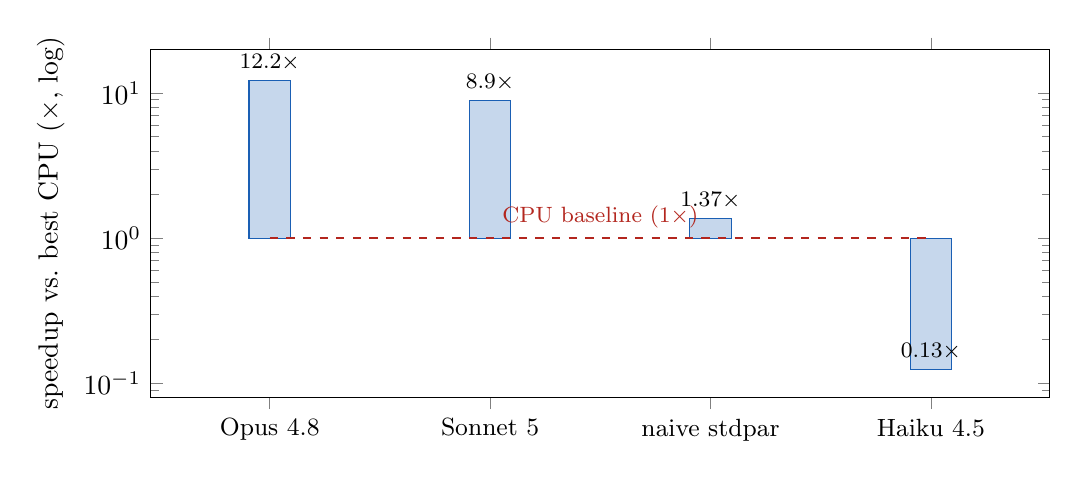
\begin{tikzpicture}
\begin{axis}[
  width=13cm, height=6cm, ymode=log,
  ybar, bar width=15pt,
  ymin=0.08, ymax=20,
  ylabel={speedup vs.\ best CPU ($\times$, log)},
  symbolic x coords={Opus 4.8, Sonnet 5, naive stdpar, Haiku 4.5},
  xtick=data, x tick label style={font=\small},
  nodes near coords, nodes near coords style={font=\footnotesize},
  point meta=explicit symbolic,
  enlarge x limits=0.18,
]
\addplot[draw=accent, fill=accent!25] coordinates {
  (Opus 4.8, 12.2) [12.2$\times$]
  (Sonnet 5, 8.9)  [8.9$\times$]
  (naive stdpar, 1.37) [1.37$\times$]
  (Haiku 4.5, 0.125) [0.13$\times$]
};
\draw[bad, thick, dashed] (axis cs:Opus 4.8,1) -- (axis cs:Haiku 4.5,1)
  node[pos=0.5, above, font=\footnotesize, text=bad] {CPU baseline ($1\times$)};
\end{axis}
\end{tikzpicture}
\caption{Speedup of each accepted port and of the naive compiler-only GPU
attempt, relative to the best CPU build. Above the dashed line is faster than the
CPU; Haiku's correct-but-slow port sits below it.}
\label{fig:speedup}
\end{figure}

\begin{figure}[htbp]
\centering
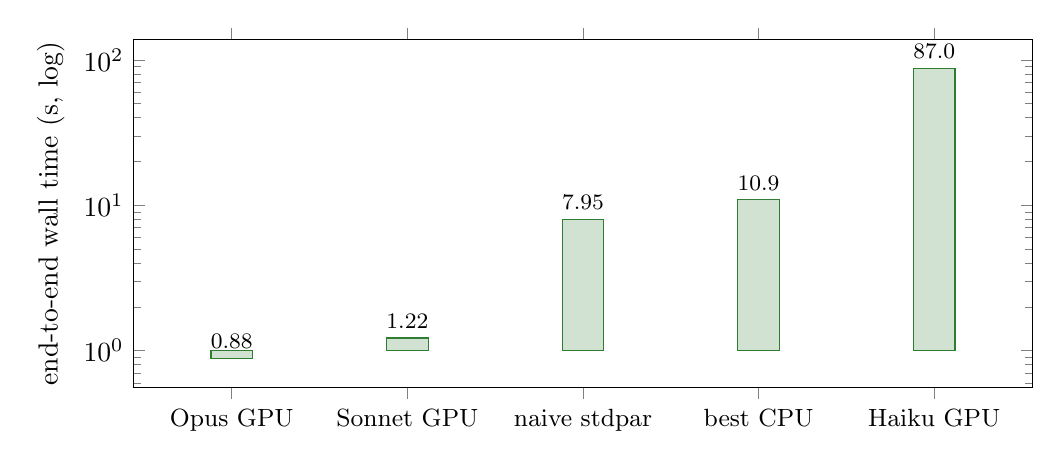
\begin{tikzpicture}
\begin{axis}[
  width=13cm, height=6cm, ymode=log,
  ybar, bar width=15pt,
  ylabel={end-to-end wall time (s, log)},
  symbolic x coords={Opus GPU, Sonnet GPU, naive stdpar, best CPU, Haiku GPU},
  xtick=data, x tick label style={font=\small},
  nodes near coords, nodes near coords style={font=\footnotesize},
  point meta=explicit symbolic,
  enlarge x limits=0.14,
]
\addplot[draw=good, fill=good!22] coordinates {
  (Opus GPU, 0.88) [0.88]
  (Sonnet GPU, 1.22) [1.22]
  (naive stdpar, 7.95) [7.95]
  (best CPU, 10.90) [10.9]
  (Haiku GPU, 86.97) [87.0]
};
\end{axis}
\end{tikzpicture}
\caption{Wall-clock time for the two-million-point, 5000-step run: the two fast
accepted GPU ports, the two CPU baselines, and Haiku's slow GPU port. Whole-process
time, including CUDA start-up.}
\label{fig:time}
\end{figure}

\subsection{The iteration study: twenty attempts with a 14B local model}

We then gave qwen2.5:14b, served locally through Ollama, twenty attempts on the
same task, with the repair loop strengthened so each attempt sees its own
previous failing code alongside the compiler or comparator diagnostic.
Figure~\ref{fig:qwen} shows what happened. The first three attempts failed to
compile. From the fourth attempt onward the model produced code that
\emph{compiled and launched GPU kernels}---it crossed the build barrier and
passed the device-execution proof. But it never passed the correctness oracle:
seventeen consecutive attempts produced plausible, compiling, GPU-executing ports
that computed the wrong answer, and the oracle rejected every one. None was
accepted.

\paragraph{What the error was.} It was not a matter of accuracy---not a rounding
or floating-point-reordering difference of a few units in the last place. In
every compiling attempt the momentum equation was \emph{correct}: the velocity
\code{u} matched the reference to a relative error of about $5\times10^{-7}$,
comfortably inside tolerance. The continuity equation was grossly \emph{wrong}:
the height \code{h} was off by up to $1.8\times10^{-2}$ in absolute terms, and by
a relative error of about $68$---thousands of percent---where the true height
passes near zero. The cause is a single indexing bug in the mass-flux stencil.
The reference takes the centered difference of the flux $u\,(hmean+h)$, so the
forward term uses the \emph{forward} velocity,
\code{u(i+1)*(hmean+h(i+1)) - u(i-1)*(hmean+h(i-1))}; the model instead paired the
\emph{centre} velocity with the forward height,
\code{u(i)*(hmean+h(i+1)) - u(i-1)*(hmean+h(i-1))}---an off-by-one on the velocity
index of the forward term, repeated in the periodic boundary cases. The port thus
solves the wrong equation. Tellingly, the error was byte-for-byte identical on
attempt~4 and attempt~20: over seventeen tries the model never localised the bug,
even though the comparator's per-variable verdict (\code{u} passes, \code{h}
fails) was in the feedback every time. This is precisely the failure the
correctness oracle exists to catch: code that compiles, runs on the device, and
produces a smooth, plausible height field while quietly solving the wrong physics.

This is the clearest single demonstration of the design's premise. Build success
is not correctness. A model too weak to get the numerics right can still get past
the compiler and onto the device; the only thing standing between ``it built and
ran on the GPU'' and ``it is accepted'' is the oracle, and here the oracle held
the line seventeen times without a single false accept.

Generation time was $10$--$18$\,s per attempt (the model was already resident, so
there was no cold-load penalty this run); the compiling attempts also paid a
build and replay cost. The twenty attempts cost roughly five minutes of local
generation and no API spend.

\begin{figure}[htbp]
\centering
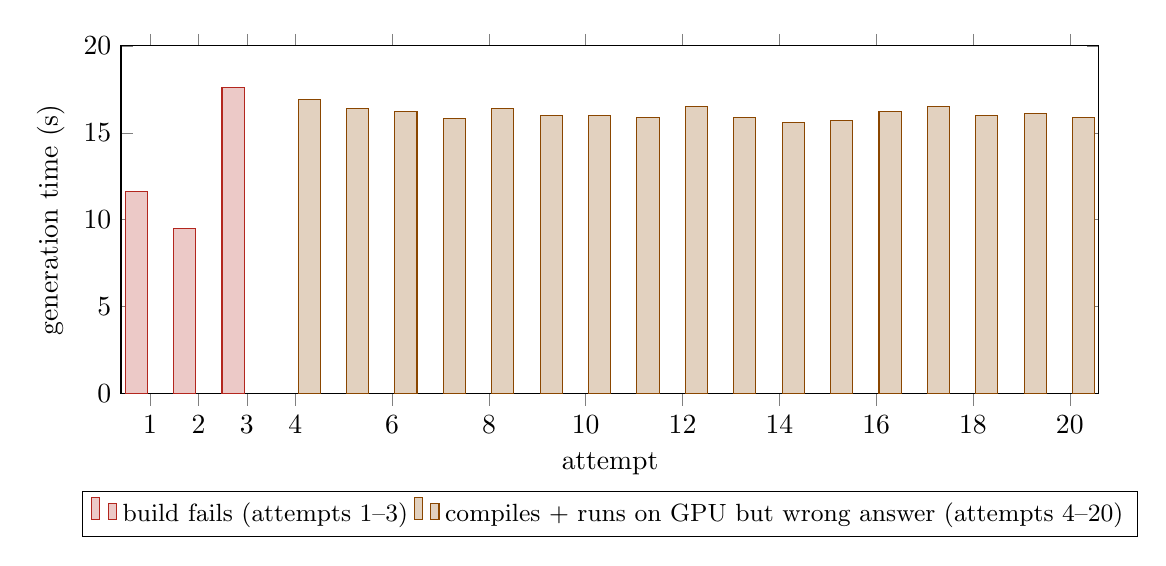
\begin{tikzpicture}
\begin{axis}[
  width=14cm, height=6cm,
  ybar, bar width=8pt,
  ymin=0, ymax=20,
  ylabel={generation time (s)}, xlabel={attempt},
  xtick={1,2,3,4,6,8,10,12,14,16,18,20},
  xmin=0.4, xmax=20.6,
  legend style={at={(0.5,-0.28)}, anchor=north, legend columns=2, font=\small},
  legend cell align=left,
]
\addplot[draw=bad, fill=bad!25] coordinates {
  (1,11.6) (2,9.5) (3,17.6)
};
\addplot[draw=warn, fill=warn!25] coordinates {
  (4,16.9) (5,16.4) (6,16.2) (7,15.8) (8,16.4) (9,16.0) (10,16.0)
  (11,15.9) (12,16.5) (13,15.9) (14,15.6) (15,15.7) (16,16.2) (17,16.5)
  (18,16.0) (19,16.1) (20,15.9)
};
\legend{build fails (attempts 1--3), compiles + runs on GPU but wrong answer (attempts 4--20)}
\end{axis}
\end{tikzpicture}
\caption{qwen2.5:14b over twenty attempts. Bar height is per-attempt generation
time. Red: the port did not compile. Amber: the port compiled and launched GPU
kernels but failed the correctness oracle. The build barrier is crossed at
attempt~4; the correctness barrier is never crossed.}
\label{fig:qwen}
\end{figure}

\section{Reading the results}

The four models span the full spectrum the harness is built to sort. Opus and
Sonnet cleared every gate and delivered eight- to twelve-fold speedups. Haiku
cleared the correctness gates but not the performance bar, and we keep that
$0.13\times$ as evidence that ``on the GPU and correct'' does not imply ``fast.''
Gemini Flash and qwen could not produce a correct port at all: Gemini stopped at
the compiler, and qwen---given twenty tries---got as far as compiling, correct-
looking, GPU-executing code that was numerically wrong, and was stopped by the
oracle every time.

The through-line is that the outcomes were decided by the harness, not asserted
by the model. Every failure landed on a specific gate---the compiler, the
device-execution proof, or the correctness oracle---and no wrong or ineffective
port was ever accepted. That is the property the skateboard exists to
demonstrate, and these early trials demonstrate it across a wide range of model
capability, two commercial APIs, and one model running locally on the same
machine.

\paragraph{Caveats.} Timings include per-process CUDA start-up. Absolute CPU
baselines drift a few percent run to run; speedups, being within-run ratios, do
not. Per-attempt wall time is measured directly only for the local model, via the
Ollama request log; for the API models we report attempt counts and the measured
end-to-end port times, not per-call latency. The correctness tolerances were
calibrated from CPU compiler spread and should be re-calibrated against
\code{nvfortran} before any external claim. All runs are on one RTX~4000 Ada; no
portability across GPUs or compilers is claimed.

\end{document}
